\documentclass[a4paper,11pt] {article}
\usepackage{graphicx}
\usepackage{amssymb, amsmath, amsthm}
\usepackage{setspace}
\usepackage{amsfonts}
%\usepackage{algorithm}
%\usepackage[noend]{algpseudocode}

%-----------Margin, Linespread, Spacing-----------%
\usepackage[letterpaper, margin=1.3in]{geometry}
\usepackage[letterpaper]{geometry}
\linespread{1}
%-------------------------------------------------%

%-----------Define header and footnotes-----------
\usepackage{fancyhdr}               % Header and footnotes
\pagestyle{fancy}
\lhead{\bfseries \scriptsize CQF}
\chead{\bfseries \scriptsize Module 3 Solution}
\rhead{\bfseries \scriptsize Ran Zhao}
\renewcommand{\headrulewidth}{0.4pt}
%-------------------------------------------------%

%---------------------Listings--------------------%
\usepackage{listings}
\usepackage{color}
\definecolor{dkgreen}{rgb}{0,0.6,0}
\definecolor{gray}{rgb}{0.5,0.5,0.5}
\definecolor{mauve}{rgb}{0.58,0,0.82}
\lstset{
  language=Octave,                % the language of the code
  basicstyle=\footnotesize,           % the size of the fonts that are used for the code
  numbers=left,                   % where to put the line-numbers
  numberstyle=\tiny\color{gray},  % the style that is used for the line-numbers
  stepnumber=2,                   % the step between two line-numbers. If it's 1, each line
                                  % will be numbered
  numbersep=5pt,                  % how far the line-numbers are from the code
  backgroundcolor=\color{white},      % choose the background color. You must add \usepackage{color}
  showspaces=false,               % show spaces adding particular underscores
  showstringspaces=false,         % underline spaces within strings
  showtabs=false,                 % show tabs within strings adding particular underscores
  frame=single,                   % adds a frame around the code
  rulecolor=\color{black},        % if not set, the frame-color may be changed on line-breaks within not-black text (e.g. commens (green here))
  tabsize=2,                      % sets default tabsize to 2 spaces
  captionpos=b,                   % sets the caption-position to bottom
  breaklines=true,                % sets automatic line breaking
  breakatwhitespace=false,        % sets if automatic breaks should only happen at whitespace
  title=\lstname,                   % show the filename of files included with \lstinputlisting;
                                  % also try caption instead of title
  keywordstyle=\color{blue},          % keyword style
  commentstyle=\color{dkgreen},       % comment style
  stringstyle=\color{mauve},         % string literal style
  escapeinside={\%*}{*)},            % if you want to add LaTeX within your code
  morekeywords={*,...}               % if you want to add more keywords to the set
}
%-------------------------------------------------%

\makeatletter
\def\BState{\State\hskip-\ALG@thistlm}
\makeatother

%----------------Title, Author, Dates-------------
\author{Ran Zhao}
\title{Asian Option Pricing using Monte Carlo Simulation}
\date{}
\begin{document}
\maketitle
%--------------------------------------------------


\section{Stock Price Simulation}
\subsection{Milstein Scheme Simulation}
The underlying stock price follows the Geometric Brownian Motion (GBM), whose dynamic is

\begin{equation} \label{eqn::GBM}
dS_t = r_t S_t dt + \sigma_t dW_t
\end{equation}
where $r_t$ is the short rate at time $t$, and $\sigma_t$ is the implied volatility at time $t$. $W_t$ is the Wiener process.

The Forward Euler-Maruyama methods for the GBM gives

$$
S_{t+\Delta t} - S_t = r_t S_t \Delta t + \sigma_t \phi \sqrt{\Delta t}
$$
where $\Delta t$ refers to as the time step in discrete time. And $\phi$ is a standard normal random number. That is, $\phi \sim N(0,1)$.

The Milstein method corrects the Forward Euler-Maruyama with a term on error level of $O(\delta t)$. Given a stochastic process $Y_t$ with

$$
dY_t = A(Y_t,t) dt + B(Y_t,t)dW_t
$$

the discretization using Milstein scheme is

$$
Y_{t+\Delta t} - Y_t = A \Delta t + B\phi \sqrt{\Delta t} + \frac{1}{2} B \frac{\partial B}{\partial Y_t} (\phi^2 - 1) \Delta t
$$
where $\frac{1}{2}(\phi^2 - 1) \Delta t$ is the Milstein correction term. For GBM, the Milstein scheme yields

$$
S_{t+\Delta t} - S_t = r_t S_t \Delta t + \sigma_t S_t \phi \sqrt{\Delta t} + \frac{1}{2} S_t \sigma^2 (\phi^2-1) \Delta t
$$

\subsection{Antithetic Variance Reduction}
The antithetic variable technique attempts to reduce the variance by introducing negatively correlated random numbers between pair of observations. While simulating the GBM, one set of standard normal random numbers is generated, labeled as $\phi^{n} \sim N(0,1)$. Then $-\phi^{n}$ also has a standard normal distribution. Regular normal random number generating methods include Box-Muller method and Polar-Marsaglia method.

The pairs $\{(\phi^{n},-\phi^{n})\}$ are distributed more desirable than $2n$ independent samples, since the samples with antithetic variable have mean 0 and negative correlation.

%The whole simulation procedure is shown in Algorithm~\ref{alg:esg}.

%\begin{algorithm}
%\caption{Stock Price Generation}\label{alg:esg}
%\begin{algorithmic}[1]
%\Procedure{$S_T$ Projection}{$S_0,T-t,\sigma,r$} %\Comment{The g.c.d. of a and b}
%\State $S_1(0,:) = S_0$, $S_2(0,:) = S_0$
%\State $N = (T-t)/\Delta t$ \Comment{Define number of time steps}
%\For{$i=1$ to $N$} %\Comment{We have the answer if r is 0}
%\For{$\omega=1$ to $M$}    \Comment{Define number of scenarios}
%\State Generate $\phi$
%\State $S_1(i,\omega)= S_1(i-1,\omega) * (1 + r * \Delta t + \sigma * \phi * \sqrt{\Delta t} + \frac{1}{2} * \sigma^2 *(\phi^2-1)*\Delta t)$
%\State $S_2(i,\omega)= S_2(i-1,\omega) * (1 + r * \Delta t + \sigma * (-\phi) * \sqrt{\Delta t} + \frac{1}{2} * \sigma^2 *(\phi^2-1)*\Delta t)$
%\EndFor
%\EndFor %\label{euclidendwhile}
%\State \textbf{return} $\{S_1, S_2\}$  %\Comment{The gcd is b}
%\EndProcedure
%\end{algorithmic}
%\end{algorithm}

In this report, the input parameters for the simulation are set as $S0 = 100$, $E = 100$, $T-t=1$, $\Delta t = 1/365$, $\sigma = 20\%$, $r = 5\%$ and $\omega = 1000$. Therefore, each time step represents a time increment of one calendar day, and there will be 2000 scenarios/paths of underlying stock price using antithetic variable.

\subsection{Simulation Testing}
Before being used into the Asian option pricing, the stock price simulations need to be tested to ensure their mathematical or statistical properties. The main testings focus on the normal random number generation and martingale property of the underlying stock price.

Figure~\ref{fig::esg_test} presents the main testing results on the simulated stock price dynamics. The left graph plots one particular (randomly selected) stock price path over the simulation period. The stock price is simulated using Milstein scheme, where there is a correction term on the order of $O(\Delta t)$. The middle graph testifies the distribution of the random numbers that simulate the Wiener process $W_t$. The blue mark draws the empirical QQ plot of the random numbers used in the stock price simulation, which is compared to the standard normal distribution QQ plot (red line). The blue labels are within a reasonable range around the red line, which indicates that the random numbers approximately follow the standard normal distribution.

The right graph plots the averaged discounted stock price over each simulation periods. The theoretical base of this testing is the martingale property of the risk neutral pricing, that is

$$
\mathbb{E}\left[e^{-\int_0^t r_s ds}S_t\right] = S_0
$$

Hence the expected value of the discounted stock price should be $S_0$. In the right graph of Figure~\ref{fig::esg_test}, the blue line is then (equally) averaged discounted stock price at each time period, and the red line is the reference line at $S_0$ level. The comparison graph shows that the simulated stock prices are within the range of $[99.8,100.2]$, which is $\pm 0.2$ around $S_0$. The simulations pass the martingale test.

\begin{figure}
  \centering
  % Requires \usepackage{graphicx}
  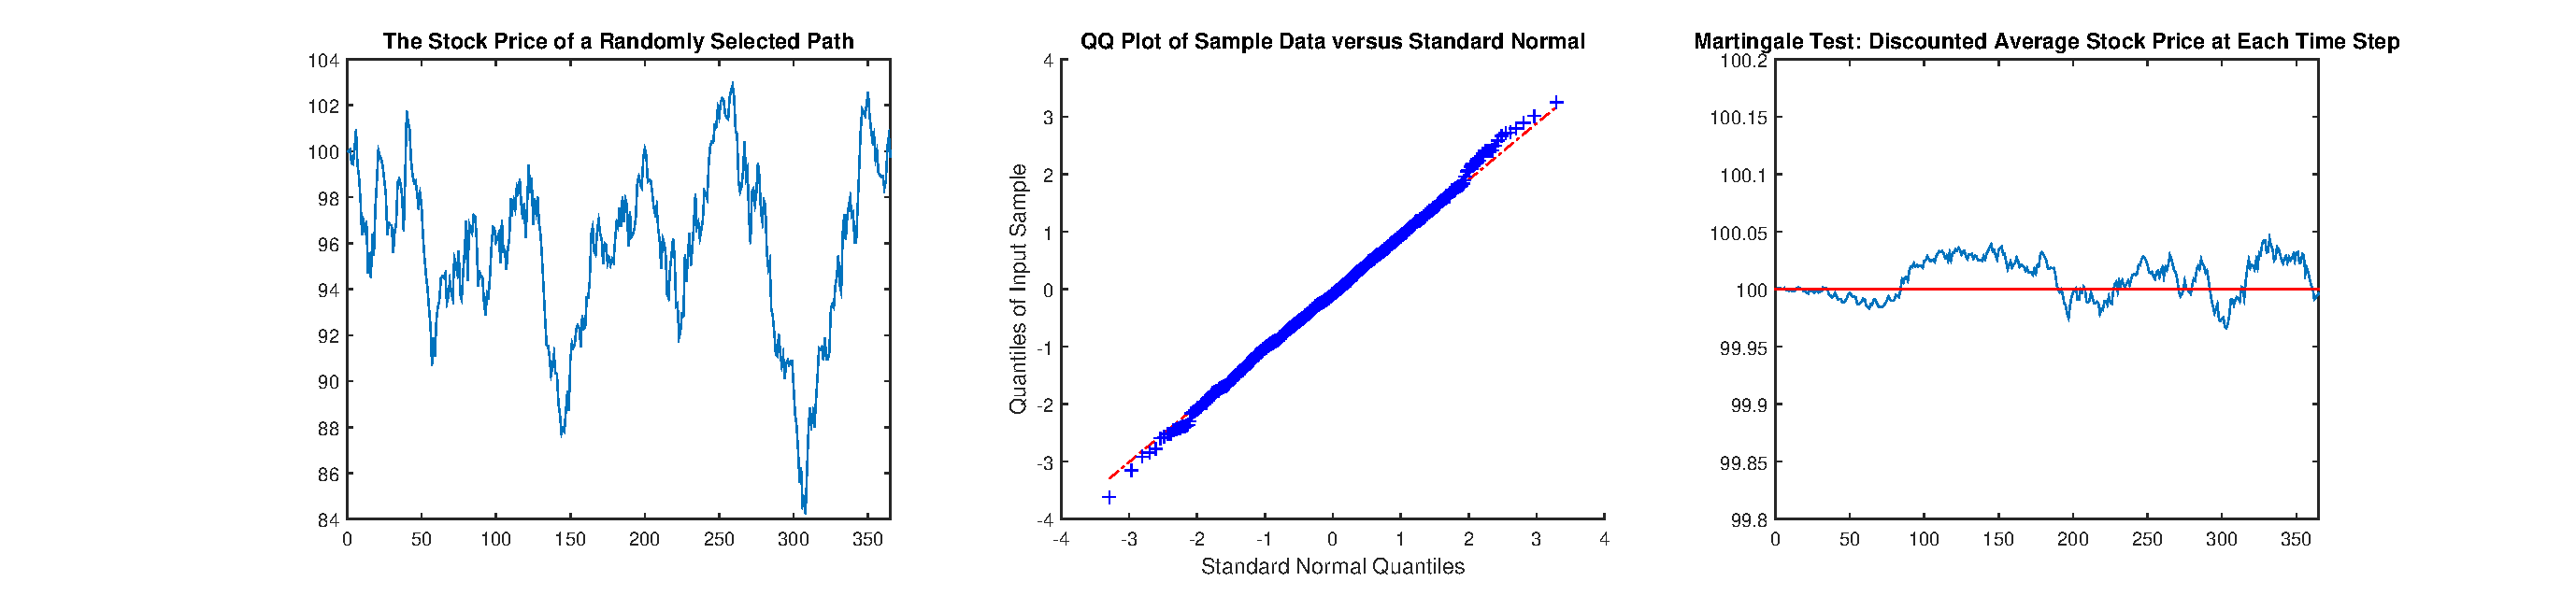
\includegraphics[scale=0.36]{esg_test.eps}\\
  \caption{The testings on the stock price simulation, including plot of a randomly selected stock price path (left), QQ plot of the random numbers for the same scenario (middle) and discounted stock price over the simulation period (right).}\label{fig::esg_test}
\end{figure}


\section{Asian Option Pricing}
\subsection{Payoff Scheme}
In general, the expected value of the discounted payoff under the risk neutral density $\mathbb{Q}$ is

$$
V(S(T),T) = \mathbb{E}^{\mathbb{Q}} \left[e^{-\int_t^T r_\tau d\tau} \textrm{\bf Payoff } (S(T)) \right]
$$

The payoff of the Asian option varies on option type (Call vs. Put), averaging method (Arithmetic vs. Geometric sampling) and strike scheme (Fixed vs. Floating strike) and so on. This report mainly discuss the option pricing differences on averaging methods and strike schemes.

\subsubsection{Averaging Method}
Consider a regular fixed strike Asian option. An Asian call option pays out
$$
C(T) = \max(A(0,T)-K,0)
$$
where $A(0,T)$ is the averaged underlying price over the period $[0,T]$.

Under arithmetic averaging scheme, the continuous time formula of the average is
$$
A(0,T) = \frac{1}{T} \int_0^T S(t)dt
$$

In discrete time, the arithmetic average is
$$
A(0,T) = \frac{1}{N} \sum_{i=0}^{N-1} S(t_i) \qquad t_i = i \cdot \frac{T}{N}
$$

Under geometric averaging scheme, the continuous time formula of the average is
$$
A(0,T) = \exp\left(\frac{1}{T} \int_0^T \ln(S(t))dt\right)
$$



\subsubsection{Strike Scheme}

\subsection{Comparison with Theoretical Price}

\section{Extensions}

%\section*{Matlab code}
%\begin{spacing}{0.9}
%\lstinputlisting[language=Matlab]{parta.m}
%\end{spacing}

\end{document} 